
\section{Introduction}
\label{sec:introduction}

% state the learning objective

%115 words
The main objective of this laboratory assignment is to study the following circuit. For that we will be using two methods that we learn in class, the mesh method and the nodal method. We decide to separate this work in other three sections, in the first one,~\ref{sec:analysis}, we will explain the theoretical analysis of this circuit, the methods that we use to analyze it and show the math tools that we use in Octave. Using Ngspice tools, in second section (\ref{sec:simulation}), we will present a simulation of our circuit and compare it with the previous results. In the last one, ~\ref{sec:conclusion}, we will summarize what we did and discuss the results.

\lipsum[1-1]



\begin{figure}[h] \centering
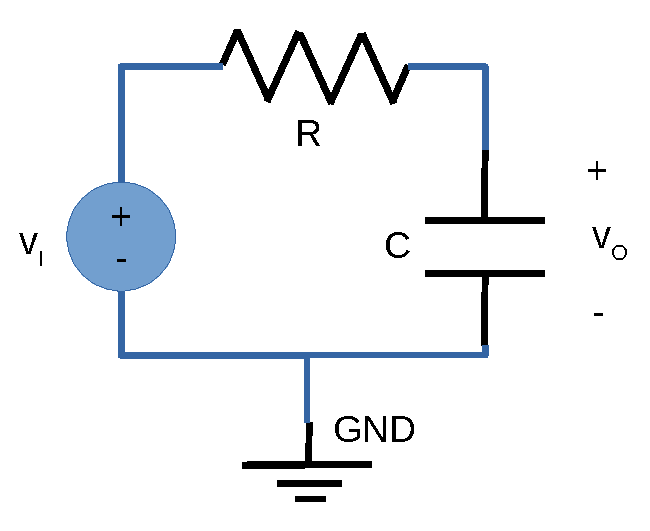
\includegraphics[width=0.4\linewidth]{rc.pdf}
\caption{Voltage driven serial RC circuit.}
\label{fig:rc}
\end{figure}
